% 第3章第1节：紧算子与有限秩逼近（紧算子与收敛改善、有限秩逼近与算子范数）。

\section{紧算子与有限秩逼近}
\label{sec:ose-compact}

本节固定一个有界线性算子，问它把有界的输入族变成怎样的输出族。有界性只保证输出也有界；在无限维空间中，有界序列未必有收敛子列，所以“有界”还不足以让输出可以被有限多个代表近似。第~\ref{sec:ose-compact-def}小节从有限秩算子出发定义紧性，并说明它怎样把弱收敛的输入变成范数收敛的输出；第~\ref{sec:ose-finite-rank}小节说明紧性在算子范数极限下保持，并在Hilbert空间中把紧算子刻画为有限秩算子的极限。

\subsection{紧算子与收敛改善}
\label{sec:ose-compact-def}

\paragraph{有限秩算子的启发}
先看输出落在有限维空间中的情形。设$X,Y$为赋范空间，有界线性算子$F:X\to Y$的像$\operatorname{Ran}F$是有限维子空间，称$F$为\term{有限秩算子}（finite-rank operator），$\dim\operatorname{Ran}F$称为它的秩。取$\operatorname{Ran}F$的一组基$y_1,\ldots,y_r$，每个输出可以唯一写成$Fx=\sum_{i=1}^{r}\ell_i(x)y_i$，其中系数$\ell_i(x)$随$x$线性变化；由于有限维空间上的范数都等价，$\ell_i$都是有界线性泛函。

若$(x_n)$是$X$中满足$\|x_n\|\leq C$的有界序列，则$\|Fx_n\|\leq\|F\|C$，输出序列落在有限维空间的一个有界集合里。有限维空间中有界序列总有收敛子列（Bolzano–Weierstrass定理），因此$(Fx_n)$有范数收敛的子列。换句话说，有限秩算子把任意有界输入族压成一个“几乎有限”的输出族：只用有限个代表点，就能以任意精度覆盖全部输出。

\paragraph{紧算子的定义}
无限维的输出也可能具有同样的性质。$\ell^2$上的$A(x_n)=(x_n/n)$不是有限秩的，但它把单位球$B=\{x:\|x\|\leq1\}$压进一个越来越扁的集合：输出$y=Ax$满足$|y_n|=|x_n|/n\leq1/n$。图~\ref{fig:ose-compact-ellipse}(a)在前两个坐标张成的平面上画出单位圆及其像，像是半轴为$1$与$1/2$的椭圆；图~\ref{fig:ose-compact-ellipse}(b)显示在所有坐标方向上，像集的“半轴”$1/n$趋于零。从这个集合中取出的任意序列，前有限个坐标可以逐个抽取收敛子列，而尾部坐标被$1/n$统一压小，于是整列也能抽出收敛子列。下面把这一性质取作定义。

\begin{figure}[!htb]
  \centering
  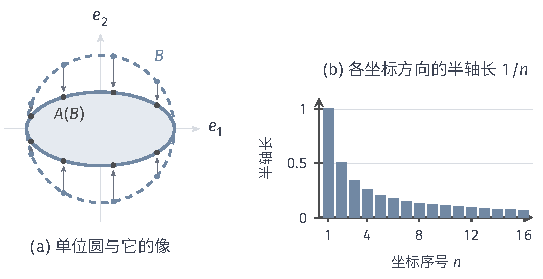
\includegraphics[width=91.9mm]{figures/02-abstract-mathematics/03-function-spaces/tikz/c3-compact-ellipse/figure.pdf}
  \caption{$\ell^2$上的$A(x_n)=(x_n/n)$怎样压缩单位球$B$。(a) 在$e_1,e_2$张成的平面上，虚线单位圆上的点沿箭头映到实线椭圆，椭圆半轴为$1$与$1/2$。(b) 像集$A(B)$的第$n$个坐标不超过$1/n$；越靠后的方向被压得越扁，这正是像集可以被有限个代表点近似覆盖的原因。}
  \label{fig:ose-compact-ellipse}
\end{figure}

\begin{definition}[紧算子]
\label{def:ose-compact-operator}
设$X,Y$为赋范空间，$A:X\to Y$为线性算子。若对$X$中每个有界序列$(x_n)$，输出序列$(Ax_n)$都有在$Y$中按范数收敛的子列，则称$A$为\term{紧算子}（compact operator）。等价地，单位球的像$A(B)$在$Y$中相对紧，即其闭包是紧集。
\end{definition}

紧算子必然有界：若$A$无界，可取单位向量$x_n$使$\|Ax_n\|\geq n$，输出序列的任何子列都无界，不可能收敛。由前面的讨论，每个有界有限秩算子都是紧算子。$A(x_n)=(x_n/n)$的紧性在第~\ref{sec:ose-finite-rank}小节用有限秩逼近给出简洁的证明。

\paragraph{单位算子不紧}
紧性不是每个有界算子都具备的。设$H$为无限维Hilbert空间，取标准正交序列$(e_n)$。对$n\neq m$，由正交性，
\[
  \|e_n-e_m\|^2=\|e_n\|^2+\|e_m\|^2=2 .
\]
单位算子$I$把这个有界序列原样输出，任意两项相距$\sqrt2$，任何子列都不是柯西列，因而没有收敛子列，$I$不是紧算子。同样的序列经过$A(x_n)=(x_n/n)$后变成$Ae_n=e_n/n$，它按范数趋于零。图~\ref{fig:ose-identity-orthonormal}对比了两种输出：左图中三个正交方向两两相距$\sqrt2$，而它们在$A$下的像向原点收拢；右图显示相邻输出的距离在单位算子下恒为$\sqrt2$，在$A$下逐渐趋于零。

\begin{figure}[!htb]
  \centering
  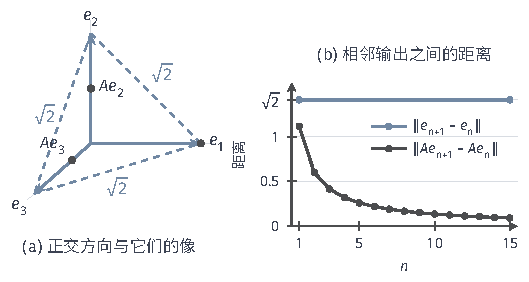
\includegraphics[width=89.6mm]{figures/02-abstract-mathematics/03-function-spaces/tikz/c3-identity-orthonormal/figure.pdf}
  \caption{同一个标准正交序列经过单位算子与经过$A(x_n)=(x_n/n)$的对比。(a) $e_1,e_2,e_3$两两相距$\sqrt2$（虚线），它们在$A$下的像$Ae_1=e_1$、$Ae_2=e_2/2$、$Ae_3=e_3/3$（黑点）向原点收拢。(b) 相邻输出的距离：单位算子下恒为$\sqrt2$，在$A$下等于$\sqrt{1/n^2+1/(n+1)^2}$并趋于零。}
  \label{fig:ose-identity-orthonormal}
\end{figure}

这个例子还提醒我们紧性约束的是什么。由第~\ref{sec:fs-orthogonal-expansion}节，每个$x\in H$都能被它在前$n$个基向量上的截断任意逼近；单独看每个函数，“有限截断”都可行。紧性要求的却是：同一个算子作用于整个有界输入族之后，输出整体可以被有限个代表覆盖。单位算子对每个输入都能截断，对整个单位球却不能，二者的差别正是逐个逼近与统一逼近的差别。

\paragraph{紧算子把弱收敛改善为范数收敛}
第~\ref{sec:lfo-weak-convergence}节已经看到，标准正交序列$e_n\rightharpoonup0$却不按范数收敛。上面的例子中，$Ae_n=e_n/n$按范数收敛到$A0=0$；这不是巧合，紧算子总能把弱收敛的输入变成按范数收敛的输出。

\begin{theorem}[紧算子改善收敛]
\label{thm:ose-compact-weak-strong}
设$X,Y$为赋范空间，$A:X\to Y$为紧算子。若$x_n\rightharpoonup x$，则$\|Ax_n-Ax\|\to0$。
\end{theorem}

\begin{proof}
第一步，说明输入有界、输出弱收敛。由第~\ref{sec:lfo-weak-norm}节，弱收敛序列有界，设$\sup_n\|x_n\|=C<\infty$。对每个$\ell\in Y^*$，复合$\ell\circ A$是$X$上的有界线性泛函，所以$\ell(Ax_n)=(\ell\circ A)(x_n)\to(\ell\circ A)(x)=\ell(Ax)$，即$Ax_n\rightharpoonup Ax$。这一步只用到$A$有界。

第二步，用反证法加上紧性。假设$Ax_n$不按范数收敛到$Ax$，则存在$\varepsilon>0$及子列$(x_{n_k})$，使$\|Ax_{n_k}-Ax\|\geq\varepsilon$对所有$k$成立。子列$(x_{n_k})$仍有界，由紧性可再抽出子列，使相应输出按范数收敛到某个$y\in Y$。

第三步，确认这个极限只能是$Ax$。范数收敛蕴含弱收敛，所以沿这个更细的子列，输出同时弱收敛到$y$和$Ax$。由第~\ref{sec:lfo-hahn-banach}节，连续线性泛函可以区分$Y$中不同的点，故弱极限唯一，$y=Ax$。这与$\|Ax_{n_k}-Ax\|\geq\varepsilon$矛盾。
\end{proof}

证明的分工很清楚：有界性只给出弱收敛被保持，紧性提供范数收敛的子列，弱极限的唯一性再把所有子列的极限钉在同一点。对一般有界算子，第二步不成立：单位算子把$e_n\rightharpoonup0$原样输出，输出仍只是弱收敛。

\subsection{有限秩逼近与算子范数}
\label{sec:ose-finite-rank}

上一小节的例子暗示，紧算子可以看作“有限秩算子的极限”。本小节把这一直觉分成两个方向：先证明紧算子的算子范数极限仍是紧算子，这给出构造紧算子的方法；再在Hilbert空间中证明反方向，即每个紧算子都能由有限秩算子按算子范数逼近。

\paragraph{算子范数极限保持紧性}
证明要用到第~\ref{sec:metric-complete-totally-bounded}节的定理~\ref{thm:metric-compact-complete-tb}：度量空间紧致当且仅当它完备且全有界，全有界指对每个$\varepsilon>0$都能被有限个半径$\varepsilon$的球覆盖。在完备空间$Y$中，全有界集合的闭包仍全有界，又作为闭子集完备，因而是紧集；所以要证像集相对紧，只需证它全有界。

\begin{theorem}[紧算子集合在算子范数下闭]
\label{thm:ose-compact-limit}
设$X$为赋范空间，$Y$为Banach空间，$A_n:X\to Y$都是紧算子，$A\in\mathcal B(X,Y)$且$\|A_n-A\|\to0$，则$A$是紧算子。
\end{theorem}

\begin{proof}
只需证明单位球的像$A(B)$全有界，再用$Y$的完备性得到闭包紧。给定$\varepsilon>0$，先取$n$使$\|A_n-A\|<\varepsilon$。由于$A_n$紧，$A_n(B)$全有界，存在有限个点$y_1,\ldots,y_N\in Y$，使每个$A_nx$（$x\in B$）都满足$\min_i\|A_nx-y_i\|<\varepsilon$。

对任意$x\in B$，选出相应的$y_i$，用三角不等式把误差拆成两段：
\[
  \|Ax-y_i\|\leq\|(A-A_n)x\|+\|A_nx-y_i\|<\|A-A_n\|\,\|x\|+\varepsilon<2\varepsilon .
\]
因此同一组$y_1,\ldots,y_N$是$A(B)$的有限$2\varepsilon$网。$\varepsilon$任意，$A(B)$全有界；$Y$完备，故$\overline{A(B)}$紧，$A$是紧算子。
\end{proof}

关键在于误差界$\|A-A_n\|$对单位球中的所有输入一致成立，于是$A_n$的有限覆盖可以整体搬给$A$。若只知道$A_nx\to Ax$对每个$x$成立，就无法这样搬运；第~\ref{sec:lfo-operator-convergence}节中投影$P_n\to I$逐点成立，而极限$I$恰好不紧。

\begin{example}[对角算子的有限秩逼近]
\label{ex:ose-diagonal-finite-rank}
在$\ell^2$上令$A(x_n)=(x_n/n)$，并令$A_m$只保留前$m$个坐标：$A_mx=(x_1,x_2/2,\ldots,x_m/m,0,0,\ldots)$。$A_m$的像落在前$m$个坐标张成的空间中，是有限秩算子。差$(A-A_m)x$只剩第$m+1$个坐标以后的部分，
\[
  \|(A-A_m)x\|^2=\sum_{n>m}\frac{|x_n|^2}{n^2}\leq\frac{1}{(m+1)^2}\sum_{n>m}|x_n|^2\leq\frac{\|x\|^2}{(m+1)^2},
\]
取$x=e_{m+1}$时等号成立，所以$\|A-A_m\|=1/(m+1)\to0$。由定理~\ref{thm:ose-compact-limit}，$A$是紧算子。
\end{example}

图~\ref{fig:ose-finite-rank-error}把这个误差与单位算子的截断作比较。若用坐标投影$P_m$去逼近单位算子，取$x=e_{m+1}$可知$\|I-P_m\|=1$，无论保留多少坐标，统一误差都不下降；对固定的$x$，误差$\|(I-P_m)x\|$却趋于零，只是趋于零的速度依赖$x$本身。对角算子$A$的截断误差则按$1/(m+1)$对所有单位输入同时下降。

\begin{figure}[!htb]
  \centering
  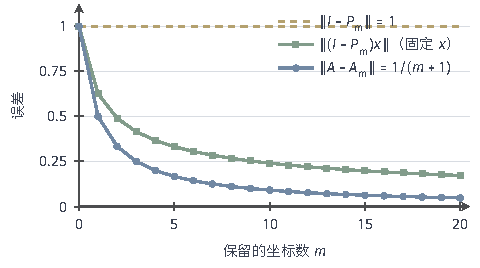
\includegraphics[width=81.2mm]{figures/02-abstract-mathematics/03-function-spaces/tikz/c3-finite-rank-error/figure.pdf}
  \caption{$\ell^2$上三种截断误差随保留坐标数$m$的变化。虚线：单位算子的统一误差$\|I-P_m\|$恒为$1$。方点：固定单位向量$x\propto(1/n)$的误差$\|(I-P_m)x\|$趋于零，但这一速度只属于这个$x$。圆点：紧算子$A(x_n)=(x_n/n)$的统一误差$\|A-A_m\|=1/(m+1)$。}
  \label{fig:ose-finite-rank-error}
\end{figure}

\paragraph{Hilbert空间中紧算子的有限秩逼近}
现在证明反方向。思路是：紧算子的像集可以被有限个点覆盖，这些点张成一个有限维子空间；向这个子空间作正交投影，就得到一个有限秩近似。正交投影的最近点性质（第~\ref{sec:fs-projection}节）保证投影误差不超过到覆盖点的距离。

\begin{theorem}[紧算子的有限秩逼近]
\label{thm:ose-finite-rank-approx}
设$X$为赋范空间，$H$为Hilbert空间，$A:X\to H$为紧算子。则存在有限秩算子$A_n:X\to H$，使$\|A-A_n\|\to0$。
\end{theorem}

\begin{proof}
给定$\varepsilon>0$。由紧性，$A(B)$全有界，取有限个点$y_1,\ldots,y_N$构成$A(B)$的$\varepsilon$网。令$M=\operatorname{span}\{y_1,\ldots,y_N\}$，它是有限维子空间，因而闭；设$P$为到$M$的正交投影，并令$F=PA$。$F$的像含于$M$，且$\|F\|\leq\|P\|\|A\|=\|A\|$，所以$F$是有界有限秩算子。

对任意$x\in B$，选$y_i$使$\|Ax-y_i\|<\varepsilon$。由于$PAx$是$M$中离$Ax$最近的点，而$y_i\in M$，
\[
  \|Ax-Fx\|=\|Ax-PAx\|\leq\|Ax-y_i\|<\varepsilon .
\]
对$x\in B$取上确界得$\|A-F\|\leq\varepsilon$。令$\varepsilon=1/n$，即得所需的有限秩算子列。
\end{proof}

证明中真正用到的是Hilbert空间的正交投影：它把有限覆盖转化为一个有界线性的“取最近点”操作。在一般Banach空间中，有限维子空间上不一定存在范数可控的投影，紧算子能否由有限秩算子按算子范数逼近，取决于空间是否具有所谓的逼近性质；确实存在不具有这一性质的Banach空间，所以本定理不能无条件推广。结合定理~\ref{thm:ose-compact-limit}，在Hilbert空间之间，紧算子恰好是有限秩算子的算子范数极限。后面的积分核逼近（第~\ref{sec:ose-hilbert-schmidt}节）和Fredholm二择的证明（第~\ref{sec:ose-fredholm}节）都会用到这一刻画。
